\documentclass[12pt,a4paper]{article}

% ===== Codificación y español =====
\usepackage[utf8]{inputenc}
\usepackage[T1]{fontenc}
\usepackage[spanish, es-tabla]{babel}

% ===== Márgenes y gráficos =====
\usepackage{geometry}
\geometry{margin=2.5cm}
\usepackage{graphicx}
\usepackage{float}        % [H] para fijar figuras/tablas
\usepackage{subcaption}   % subfiguras
\usepackage{booktabs}     % tablas más bonitas

% ===== Hipervínculos y referencias =====
\usepackage{hyperref}
\hypersetup{
  colorlinks=true,
  linkcolor=black,
  citecolor=black,
  urlcolor=blue
}

\usepackage{siunitx}
\sisetup{
  output-decimal-marker = {.}, % decimal con punto
  group-separator = {,},       % miles con coma
  group-minimum-digits = 4,
  group-digits = integer,
  table-number-alignment = center,
  round-mode = places,
  detect-all = true            % ignora configuraciones de babel
}

% Ayuda al manejo de tablas
\usepackage{tabularx}
\usepackage{adjustbox}
\usepackage{longtable}

% cleveref mejora \ref: escribe "Figura 1", "Tabla 2", etc.
\usepackage[capitalise,noabbrev]{cleveref}

% Ajuste de nombres en cleveref
\crefname{figure}{figura}{figuras}
\Crefname{figure}{Figura}{Figuras}
\crefname{subfigure}{subfigura}{subfiguras}
\Crefname{subfigure}{Subfigura}{Subfiguras}
\crefname{table}{tabla}{tablas}
\Crefname{table}{Tabla}{Tablas}
\crefname{equation}{ecuación}{ecuaciones}
\Crefname{equation}{Ecuación}{Ecuaciones}
\crefname{section}{sección}{secciones}
\Crefname{section}{Sección}{Secciones}

% Listas más controlables
\usepackage{enumitem}

\graphicspath{{figures/}}

% ===== Título y autoría =====
\title{\textbf{\textit{"Playing"} con diferentes clasificadores y datasets}}
\author{Haessler Joan Ortiz Moncada \\[0.5cm]
        Universidad Distrital Francisco José de Caldas \\
        Facultad de Ingeniería \\
        Curso: Big Data}
\date{\today}

\begin{document}

\maketitle

\section{Introducción}
Este documento presenta el desarrollo del \texttt{Assignment \#4} del curso de Big Data y documenta 
los hallazgos y análisis correspondientes, haciendo uso de tres métricas e incorporando gráficos 
adecuados que permitan evidenciar y sustentar los resultados. El \texttt{Assignment \#4} propone 
experimentar con diversos modelos de clasificación sobre distintos conjuntos de datos (\texttt{Blobs}, 
\texttt{Gaussian Quartiles} y \texttt{Moons}), con diferentes tamaños de muestra y niveles de ruido 
inducido.

\section{Metodología}
Se desarrolla conforme a lo establecido en el \texttt{Assignment \#4}, aunque con algunas variaciones 
en la presentación. En aquel caso se solicitaba que todo el trabajo se realizara en un único documento o 
archivo de Colab; en cambio, aquí se optó por efectuar la codificación en dicho entorno y presentar los 
hallazgos y el compendio de resultados mediante un informe escrito. Se emplearon principalmente Google Colab y Python, 
haciendo uso de los paquetes \texttt{os}, \texttt{pandas}, \texttt{scikit-learn}, \texttt{matplotlib} y \texttt{seaborn}.
También se tuvo en cuenta manejar el mismo escenario de aleatoriedad (semiila) para poder replicar los resultados.

Básicamente, lo que se hizo fue ir desarrollando en Colab el código correspondiente y de manera 
paralela documentar los hallazgos y resultados en este informe. Por último, el código fuente implementado en Colab, 
los datos utilizados y el archivo de este informe se encuentran en la carpeta taller\_4 del repositorio de 
GitHub \href{https://github.com/HaesslerOrtiz/bigdata}{bigdata\_repositorio}.

\section{Escenario 1: binario vs. clasificación multiclase}
En esta sección se construyeron tres conjuntos de datos: uno binario (dos clases) y otros dos con cinco y veinte clases, 
respectivamente. Como el \texttt{Assignment \#4} no especificó el tamaño, se fijaron en 1,000 registros cada uno. Para 
su construcción se emplearon datos tipo \texttt{Blobs}, cuyas observaciones se distribuyen como puntos en el plano 
cartesiano; cada clase agrupa sus puntos en una región del espacio. Los datos se dividieron en entrenamiento, validación 
y prueba en proporciones de 60\%, 20\% y 20\%, respectivamente; además, se aplicó estratificación para que cada partición 
mantuviera la misma distribución de clases que el dataset padre. La \Cref{fig:hist_2_5} muestra como las frecuencias 
de las clases para el dataset binario y para el de cinco clases, mientras la \Cref{fig:hist_20} muestra la frecuencia 
del dataset que cse clasifica en 20 clases.

\begin{figure}[H]
  \centering
  \begin{subfigure}[b]{0.45\textwidth}
    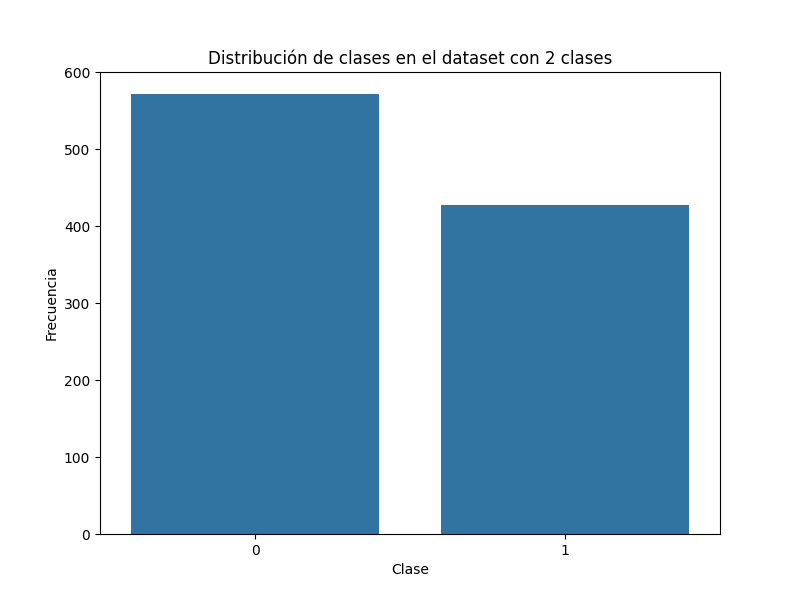
\includegraphics[width=\textwidth]{histogram_2_classes.png}
    \caption{Frecuencia clases dataset binario.}
    \label{fig:hist_2}
  \end{subfigure}
  \hfill
  \begin{subfigure}[b]{0.45\textwidth}
    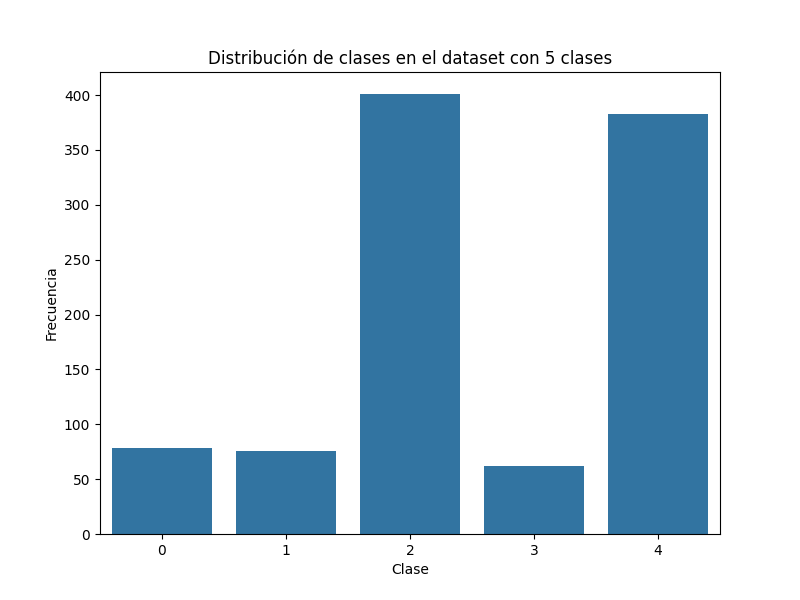
\includegraphics[width=\textwidth]{histogram_5_classes.png}
    \caption{Frecuencia clases dataset de cinco clases.}
    \label{fig:hist_5}
  \end{subfigure}
  \caption{Frecuencia clases datasets binario y de cinco clases.}
  \label{fig:hist_2_5}
\end{figure}

\begin{figure}[H]
  \centering
  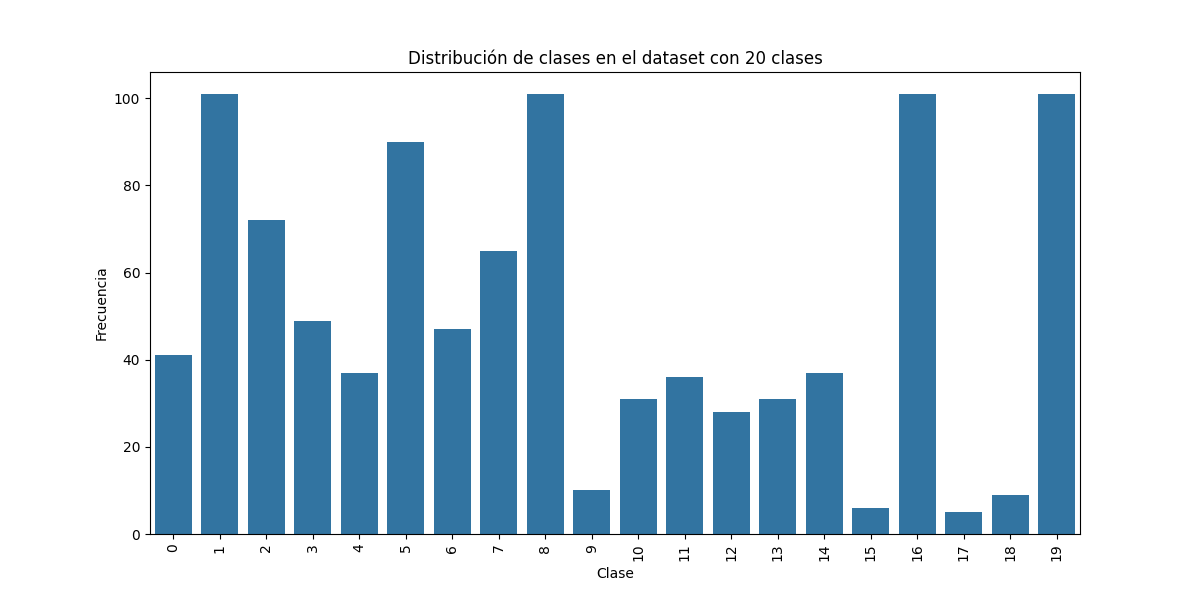
\includegraphics[width=\textwidth]{histogram_20_classes.png}
  \caption{Frecuencia clases dataset de veinte clases.}
  \label{fig:hist_20}
\end{figure}

\subsection{Probando con distintos clasificadores}
En este y en los siguientes escenarios, se evaluará cómo distintos clasificadores predicen las clases de cada conjunto de datos, 
explorando los hiperparámetros configurables de cada modelo. Posteriormente, se seleccionará la combinación de hiperparámetros 
que ofrezca el mejor desempeño predictivo según las métricas \texttt{Accuracy}, \texttt{Recall} y \texttt{F1-Score}.

\begin{enumerate}

  \item \textbf{Vecinos más cercanos (k-NN).}
  Probando con un rango de 1 a 30 vecinos para cada uno de los datasets conformados, se definio que el mejor desempeño se obtuvo 
  con los siguientes hiperparámetros:

  \begin{itemize}
    \item \textbf{Dataset binario.} 1 vecinos.
    \item \textbf{Dataset con cinco clases.} 8 vecinos.
    \item \textbf{Dataset con veinte clases.} 19 vecinos.
  \end{itemize}

  Respecto al desempeño obtenido en cada uno de los modelos se tienen los siguientes resultados:

  \small
  \setlength{\tabcolsep}{4pt}
  \begin{longtable}{@{}lcccc@{}}
    \toprule
    \textbf{Clase} & \textbf{Precision} & \textbf{Recall} & \textbf{F1-Score} & \textbf{Support} \\
    \midrule
    \endfirsthead

    \toprule
    \textbf{Clase} & \textbf{Precision} & \textbf{Recall} & \textbf{F1-Score} & \textbf{Support} \\
    \midrule
    \endhead

    \midrule
    \multicolumn{5}{r}{\emph{Continúa en la siguiente página}} \\
    \endfoot

    \bottomrule
    \caption{Reportes de clasificación k-NN en tres escenarios (2, 5 y 20 clases).}
    \label{tab:reportes_clasificacion_knn_long}
    \endlastfoot

    % ================= (a) 2 clases =================
    \multicolumn{5}{@{}l}{\textbf{(a) 2 clases}}\\
    0 & 1.00 & 1.00 & 1.00 & 115 \\
    1 & 1.00 & 1.00 & 1.00 & 85 \\
    \midrule
    \multicolumn{3}{l}{\textbf{Accuracy}} & \textbf{1.00} & 200 \\
    \textbf{Macro avg}    & 1.00 & 1.00 & 1.00 & 200 \\
    \textbf{Weighted avg} & 1.00 & 1.00 & 1.00 & 200 \\
    \addlinespace[0.8em]

    % ================= (b) 5 clases =================
    \multicolumn{5}{@{}l}{\textbf{(b) 5 clases}}\\
    0 & 1.00 & 1.00 & 1.00 & 16 \\
    1 & 0.86 & 0.80 & 0.83 & 15 \\
    2 & 1.00 & 1.00 & 1.00 & 80 \\
    3 & 1.00 & 1.00 & 1.00 & 13 \\
    4 & 0.96 & 0.97 & 0.97 & 76 \\
    \midrule
    \multicolumn{3}{l}{\textbf{Accuracy}} & \textbf{0.97} & 200 \\
    \textbf{Macro avg}    & 0.96 & 0.95 & 0.96 & 200 \\
    \textbf{Weighted avg} & 0.97 & 0.97 & 0.97 & 200 \\
    \addlinespace[0.8em]

    % ================= (c) 20 clases =================
    \multicolumn{5}{@{}l}{\textbf{(c) 20 clases}}\\
    0 & 1.00 & 1.00 & 1.00 & 8 \\
    1 & 0.91 & 1.00 & 0.95 & 20 \\
    2 & 0.67 & 0.53 & 0.59 & 15 \\
    3 & 0.80 & 0.40 & 0.53 & 10 \\
    4 & 1.00 & 1.00 & 1.00 & 7 \\
    5 & 0.52 & 0.67 & 0.59 & 18 \\
    6 & 1.00 & 1.00 & 1.00 & 9 \\
    7 & 0.56 & 0.77 & 0.65 & 13 \\
    8 & 0.83 & 1.00 & 0.91 & 20 \\
    9 & 0.00 & 0.00 & 0.00 & 2 \\
    10 & 0.75 & 1.00 & 0.86 & 6 \\
    11 & 0.71 & 0.71 & 0.71 & 7 \\
    12 & 1.00 & 1.00 & 1.00 & 6 \\
    13 & 0.75 & 0.50 & 0.60 & 6 \\
    14 & 1.00 & 0.88 & 0.93 & 8 \\
    15 & 0.00 & 0.00 & 0.00 & 1 \\
    16 & 0.65 & 0.65 & 0.65 & 20 \\
    17 & 0.00 & 0.00 & 0.00 & 1 \\
    18 & 0.00 & 0.00 & 0.00 & 2 \\
    19 & 1.00 & 0.95 & 0.98 & 21 \\
    \midrule
    \multicolumn{3}{l}{\textbf{Accuracy}} & \textbf{0.79} & 200 \\
    \textbf{Macro avg}    & 0.66 & 0.65 & 0.65 & 200 \\
    \textbf{Weighted avg} & 0.78 & 0.79 & 0.78 & 200 \\
  \end{longtable}

  \item \textbf{Arbol de decisión.}
  Se buscó la mejor configuración de hiperparámetros en el siguiente marco:
  \begin{table}[htbp]
    \centering
    \begin{tabular}{@{}lll@{}}
      \toprule
      \textbf{Parámetro} & \textbf{Descripción} & \textbf{Valores probados} \\
      \midrule
      \texttt{max\_depth} & Profundidad máxima del árbol & \{None, 5, 10, 15, 20\} \\
      \texttt{min\_samples\_split} & Mín. muestras para dividir un nodo interno & \{2, 5, 10\} \\
      \texttt{min\_samples\_leaf} & Mín. muestras por hoja & \{1, 2, 4\} \\
      \bottomrule
    \end{tabular}
    \caption{Rangos de hiperparámetros evaluados para \texttt{DecisionTreeClassifier}.}
    \label{tab:param_dt_ranges}
  \end{table}

  Con base en esta busqueda se obtuvieron las siguientes mejores configuraciones de hiperparámetros para cada dataset:

  \begin{table}[htbp]
    \centering
    \begin{tabular}{@{}lccc@{}}
      \toprule
      \textbf{Clases} & \texttt{max\_depth} & \texttt{min\_samples\_leaf} & \texttt{min\_samples\_split} \\
      \midrule
      2  & \texttt{None} & 1 & 2 \\
      5  & 5              & 1 & 2 \\
      20 & 10             & 1 & 5 \\
      \bottomrule
    \end{tabular}
    \caption{Mejores hiperparámetros encontrados para \texttt{Arbol de decisión}.}
    \label{tab:best_hparams_dt}
  \end{table}

  Respecto al desempeño obtenido en cada uno de los modelos se tienen los siguientes resultados:

  \small
  \setlength{\tabcolsep}{4pt}
  \begin{longtable}{@{}lcccc@{}}
    \toprule
    \textbf{Clase} & \textbf{Precision} & \textbf{Recall} & \textbf{F1-Score} & \textbf{Support} \\
    \midrule
    \endfirsthead

    \toprule
    \textbf{Clase} & \textbf{Precision} & \textbf{Recall} & \textbf{F1-Score} & \textbf{Support} \\
    \midrule
    \endhead

    \midrule
    \multicolumn{5}{r}{\emph{Continúa en la siguiente página}} \\
    \endfoot

    \bottomrule
    \caption{Reportes de clasificación — Árbol de decisión (2, 5 y 20 clases).}
    \label{tab:reportes_clasificacion_arbol}
    \endlastfoot

    % ================= (a) 2 clases =================
    \multicolumn{5}{@{}l}{\textbf{(a) 2 clases}}\\
    0 & 1.00 & 1.00 & 1.00 & 115 \\
    1 & 1.00 & 1.00 & 1.00 & 85 \\
    \midrule
    \multicolumn{3}{l}{\textbf{Accuracy}} & \textbf{1.00} & 200 \\
    \textbf{Macro avg}    & 1.00 & 1.00 & 1.00 & 200 \\
    \textbf{Weighted avg} & 1.00 & 1.00 & 1.00 & 200 \\
    \addlinespace[0.8em]

    % ================= (b) 5 clases =================
    \multicolumn{5}{@{}l}{\textbf{(b) 5 clases}}\\
    0 & 1.00 & 1.00 & 1.00 & 16 \\
    1 & 0.71 & 0.67 & 0.69 & 15 \\
    2 & 1.00 & 1.00 & 1.00 & 80 \\
    3 & 1.00 & 1.00 & 1.00 & 13 \\
    4 & 0.94 & 0.95 & 0.94 & 76 \\
    \midrule
    \multicolumn{3}{l}{\textbf{Accuracy}} & \textbf{0.95} & 200 \\
    \textbf{Macro avg}    & 0.93 & 0.92 & 0.93 & 200 \\
    \textbf{Weighted avg} & 0.95 & 0.95 & 0.95 & 200 \\
    \addlinespace[0.8em]

    % ================= (c) 20 clases =================
    \multicolumn{5}{@{}l}{\textbf{(c) 20 clases}}\\
    0 & 1.00 & 0.88 & 0.93 & 8 \\
    1 & 0.91 & 1.00 & 0.95 & 20 \\
    2 & 0.53 & 0.60 & 0.56 & 15 \\
    3 & 0.80 & 0.40 & 0.53 & 10 \\
    4 & 1.00 & 1.00 & 1.00 & 7 \\
    5 & 0.50 & 0.72 & 0.59 & 18 \\
    6 & 1.00 & 1.00 & 1.00 & 9 \\
    7 & 0.46 & 0.46 & 0.46 & 13 \\
    8 & 0.91 & 1.00 & 0.95 & 20 \\
    9 & 1.00 & 0.50 & 0.67 & 2 \\
    10 & 0.75 & 1.00 & 0.86 & 6 \\
    11 & 1.00 & 0.86 & 0.92 & 7 \\
    12 & 0.86 & 1.00 & 0.92 & 6 \\
    13 & 0.80 & 0.67 & 0.73 & 6 \\
    14 & 1.00 & 0.88 & 0.93 & 8 \\
    15 & 0.00 & 0.00 & 0.00 & 1 \\
    16 & 0.76 & 0.65 & 0.70 & 20 \\
    17 & 1.00 & 1.00 & 1.00 & 1 \\
    18 & 1.00 & 0.50 & 0.67 & 2 \\
    19 & 1.00 & 0.81 & 0.89 & 21 \\
    \midrule
    \multicolumn{3}{l}{\textbf{Accuracy}} & \textbf{0.79} & 200 \\
    \textbf{Macro avg}    & 0.81 & 0.75 & 0.76 & 200 \\
    \textbf{Weighted avg} & 0.81 & 0.79 & 0.79 & 200 \\
  \end{longtable}

  \item \textbf{Máquinas de vectores de soporte (SVM por sus siglas en inglés).}
  Para este clasificador se buscó la mejor configuración de hiperparámetros probando los siguientes valores:

  \begin{table}[htbp]
    \centering
    \begin{tabular}{@{}lll@{}}
      \toprule
      \textbf{Parámetro} & \textbf{Descripción} & \textbf{Valores probados} \\
      \midrule
      \texttt{C} & Parámetro de regularización. & \{0.1, 1, 10\} \\
      \texttt{kernel} & Tipo de núcleo usado por el algoritmo SVM. & \{\texttt{linear}, \texttt{rbf}\} \\
      \texttt{gamma} & Coeficiente del kernel. & \{\texttt{scale}, \texttt{auto}, 0.1, 1\} \\
      \bottomrule
    \end{tabular}
    \caption{Espacio de hiperparámetros evaluado para SVM.}
    \label{tab:param_svm_ranges}
  \end{table}
  
  Los mejores hiperparámetros encontrados para cada dataset, fueron los siguientes:

  \begin{table}[htbp]
    \centering
    \begin{tabular}{@{}lccc@{}}
      \toprule
      \textbf{Clases} & \texttt{C} & \texttt{gamma} & \texttt{kernel} \\
      \midrule
      2  & 0.1 & \texttt{scale} & \texttt{linear} \\
      5  & 0.1 & \texttt{scale} & \texttt{linear} \\
      20 & 0.1 & \texttt{scale} & \texttt{linear} \\
      \bottomrule
    \end{tabular}
    \caption{Mejores hiperparámetros SVM.}
    \label{tab:best_hparams_svm}
  \end{table}
  
  Con los mejores hiperparámetros encontrados, se obtuvieron los siguientes resultados:

  \small
  \setlength{\tabcolsep}{4pt}
  \begin{longtable}{@{}lcccc@{}}
    \toprule
    \textbf{Clase} & \textbf{Precision} & \textbf{Recall} & \textbf{F1-Score} & \textbf{Support} \\
    \midrule
    \endfirsthead

    \toprule
    \textbf{Clase} & \textbf{Precision} & \textbf{Recall} & \textbf{F1-Score} & \textbf{Support} \\
    \midrule
    \endhead

    \midrule
    \multicolumn{5}{r}{\emph{Continúa en la siguiente página}} \\
    \endfoot

    \bottomrule
    \caption{Reportes de clasificación — \textbf{SVM} (2, 5 y 20 clases).}
    \label{tab:reportes_clasificacion_svm}
    \endlastfoot

    % ================= (a) 2 clases =================
    \multicolumn{5}{@{}l}{\textbf{(a) 2 clases}}\\
    0 & 1.00 & 1.00 & 1.00 & 115 \\
    1 & 1.00 & 1.00 & 1.00 & 85 \\
    \midrule
    \multicolumn{3}{l}{\textbf{Accuracy}} & \textbf{1.00} & 200 \\
    \textbf{Macro avg}    & 1.00 & 1.00 & 1.00 & 200 \\
    \textbf{Weighted avg} & 1.00 & 1.00 & 1.00 & 200 \\
    \addlinespace[0.8em]

    % ================= (b) 5 clases =================
    \multicolumn{5}{@{}l}{\textbf{(b) 5 clases}}\\
    0 & 1.00 & 1.00 & 1.00 & 16 \\
    1 & 0.86 & 0.80 & 0.83 & 15 \\
    2 & 1.00 & 1.00 & 1.00 & 80 \\
    3 & 1.00 & 1.00 & 1.00 & 13 \\
    4 & 0.96 & 0.97 & 0.97 & 76 \\
    \midrule
    \multicolumn{3}{l}{\textbf{Accuracy}} & \textbf{0.97} & 200 \\
    \textbf{Macro avg}    & 0.96 & 0.95 & 0.96 & 200 \\
    \textbf{Weighted avg} & 0.97 & 0.97 & 0.97 & 200 \\
    \addlinespace[0.8em]

    % ================= (c) 20 clases =================
    \multicolumn{5}{@{}l}{\textbf{(c) 20 clases}}\\
    0 & 1.00 & 1.00 & 1.00 & 8 \\
    1 & 0.95 & 1.00 & 0.98 & 20 \\
    2 & 0.60 & 0.60 & 0.60 & 15 \\
    3 & 0.80 & 0.40 & 0.53 & 10 \\
    4 & 1.00 & 1.00 & 1.00 & 7 \\
    5 & 0.53 & 0.56 & 0.54 & 18 \\
    6 & 1.00 & 1.00 & 1.00 & 9 \\
    7 & 0.57 & 0.62 & 0.59 & 13 \\
    8 & 0.91 & 1.00 & 0.95 & 20 \\
    9 & 1.00 & 1.00 & 1.00 & 2 \\
    10 & 0.75 & 1.00 & 0.86 & 6 \\
    11 & 1.00 & 0.71 & 0.83 & 7 \\
    12 & 1.00 & 1.00 & 1.00 & 6 \\
    13 & 0.83 & 0.83 & 0.83 & 6 \\
    14 & 1.00 & 0.88 & 0.93 & 8 \\
    15 & 0.00 & 0.00 & 0.00 & 1 \\
    16 & 0.58 & 0.70 & 0.64 & 20 \\
    17 & 1.00 & 1.00 & 1.00 & 1 \\
    18 & 1.00 & 0.50 & 0.67 & 2 \\
    19 & 1.00 & 0.95 & 0.98 & 21 \\
    \midrule
    \multicolumn{3}{l}{\textbf{Accuracy}} & \textbf{0.81} & 200 \\
    \textbf{Macro avg}    & 0.83 & 0.79 & 0.80 & 200 \\
    \textbf{Weighted avg} & 0.82 & 0.81 & 0.81 & 200 \\
  \end{longtable}

   \item \textbf{Perceptrón multicapa (MLP por sus siglas en inglés).}
   Para este clasificador se buscó la mejor configuración de hiperparámetros probando con los siguientes valores:

   \begin{table}[htbp]
    \centering\small
    \setlength{\tabcolsep}{4pt}
    \begin{tabularx}{\linewidth}{@{}l l X@{}}
      \toprule
      \textbf{Parámetro} & \textbf{Descripción} & \textbf{Valores probados} \\
      \midrule
      \texttt{hidden\_layer\_sizes} & Tamaño(s) de capa(s) oculta(s) & \texttt{(50,)}, \texttt{(100,)}, \texttt{(50, 50)} \\
      \texttt{activation}           & Función de activación          & \texttt{tanh}, \texttt{relu} \\
      \texttt{solver}               & Optimizador para los pesos     & \texttt{adam} \\
      \texttt{alpha}                & Regularización L2              & 0.0001, 0.001 \\
      \texttt{learning\_rate\_init} & Tasa de aprendizaje inicial    & 0.001, 0.01 \\
      \texttt{max\_iter}            & Iteraciones máximas            & 200, 500 \\
      \bottomrule
    \end{tabularx}
    \caption{Espacio de hiperparámetros evaluado para MLP.}
    \label{tab:param_mlp_ranges_fit}
  \end{table}

   Con base en esta busqueda se obtuvieron las siguientes mejores configuraciones de hiperparámetros para cada dataset:

  \begin{table}[htbp]
    \centering\small
    \setlength{\tabcolsep}{4pt}
    \begin{tabularx}{\linewidth}{@{}l l l l l l l@{}}
      \toprule
      \textbf{Clases} & \textbf{\texttt{hidden\_layer\_sizes}} & \textbf{\texttt{activation}} & \textbf{\texttt{solver}} & \textbf{\texttt{alpha}} & \textbf{\texttt{learning\_rate\_init}} & \textbf{\texttt{max\_iter}} \\
      \midrule
      2  & \texttt{(50,)}     & \texttt{tanh} & \texttt{adam} & 0.0001 & 0.001 & 200 \\
      5  & \texttt{(50, 50)}  & \texttt{tanh} & \texttt{adam} & 0.0001 & 0.01  & 200 \\
      20 & \texttt{(100,)}    & \texttt{tanh} & \texttt{adam} & 0.0001 & 0.001 & 500 \\
      \bottomrule
    \end{tabularx}
    \caption{Mejores hiperparámetros MLP.}
    \label{tab:best_hparams_mlp}
  \end{table}

   Con la configuraciones de hiperparámetros encontradas, se obtuvieron los siguientes resultados:

    \small
    \setlength{\tabcolsep}{4pt}
    \begin{longtable}{@{}lcccc@{}}
      \toprule
      \textbf{Clase} & \textbf{Precision} & \textbf{Recall} & \textbf{F1-Score} & \textbf{Support} \\
      \midrule
      \endfirsthead

      \toprule
      \textbf{Clase} & \textbf{Precision} & \textbf{Recall} & \textbf{F1-Score} & \textbf{Support} \\
      \midrule
      \endhead

      \midrule
      \multicolumn{5}{r}{\emph{Continúa en la siguiente página}} \\
      \endfoot

      \bottomrule
      \caption{Reportes de clasificación — \textbf{MLP} (2, 5 y 20 clases).}
      \label{tab:mlp_reports_long}
      \endlastfoot

      % ================= (a) 2 clases =================
      \multicolumn{5}{@{}l}{\textbf{(a) 2 clases}}\\
      0 & 1.00 & 1.00 & 1.00 & 115 \\
      1 & 1.00 & 1.00 & 1.00 & 85 \\
      \midrule
      \multicolumn{3}{l}{\textbf{Accuracy}} & \textbf{1.00} & 200 \\
      \textbf{Macro avg}    & 1.00 & 1.00 & 1.00 & 200 \\
      \textbf{Weighted avg} & 1.00 & 1.00 & 1.00 & 200 \\
      \addlinespace[0.8em]

      % ================= (b) 5 clases =================
      \multicolumn{5}{@{}l}{\textbf{(b) 5 clases}}\\
      0 & 1.00 & 1.00 & 1.00 & 16 \\
      1 & 0.86 & 0.80 & 0.83 & 15 \\
      2 & 1.00 & 1.00 & 1.00 & 80 \\
      3 & 1.00 & 1.00 & 1.00 & 13 \\
      4 & 0.96 & 0.97 & 0.97 & 76 \\
      \midrule
      \multicolumn{3}{l}{\textbf{Accuracy}} & \textbf{0.97} & 200 \\
      \textbf{Macro avg}    & 0.96 & 0.95 & 0.96 & 200 \\
      \textbf{Weighted avg} & 0.97 & 0.97 & 0.97 & 200 \\
      \addlinespace[0.8em]

      % ================= (c) 20 clases =================
      \multicolumn{5}{@{}l}{\textbf{(c) 20 clases}}\\
      0 & 1.00 & 1.00 & 1.00 & 8 \\
      1 & 0.95 & 1.00 & 0.98 & 20 \\
      2 & 0.60 & 0.60 & 0.60 & 15 \\
      3 & 0.75 & 0.60 & 0.67 & 10 \\
      4 & 1.00 & 1.00 & 1.00 & 7 \\
      5 & 0.56 & 0.56 & 0.56 & 18 \\
      6 & 1.00 & 1.00 & 1.00 & 9 \\
      7 & 0.57 & 0.62 & 0.59 & 13 \\
      8 & 0.95 & 1.00 & 0.98 & 20 \\
      9 & 1.00 & 1.00 & 1.00 & 2 \\
      10 & 0.75 & 1.00 & 0.86 & 6 \\
      11 & 1.00 & 0.86 & 0.92 & 7 \\
      12 & 1.00 & 1.00 & 1.00 & 6 \\
      13 & 0.83 & 0.83 & 0.83 & 6 \\
      14 & 1.00 & 0.88 & 0.93 & 8 \\
      15 & 0.00 & 0.00 & 0.00 & 1 \\
      16 & 0.59 & 0.65 & 0.62 & 20 \\
      17 & 1.00 & 1.00 & 1.00 & 1 \\
      18 & 1.00 & 0.50 & 0.67 & 2 \\
      19 & 1.00 & 0.95 & 0.98 & 21 \\
      \midrule
      \multicolumn{3}{l}{\textbf{Accuracy}} & \textbf{0.82} & 200 \\
      \textbf{Macro avg}    & 0.83 & 0.80 & 0.81 & 200 \\
      \textbf{Weighted avg} & 0.82 & 0.82 & 0.82 & 200 \\
    \end{longtable}

  \item \textbf{Análisis de resultados.}
  
  \begin{itemize}
    \item \textbf{Tendencia general.} Con 2 clases, todos los modelos aciertan casi perfecto. Con 5 clases siguen muy altos. 
    Al pasar a \textbf{20 clases}, la exactitud baja para todos ($\approx$ 0.79--0.82) por mayor solapamiento entre clases 
    y menos ejemplos por clase.
    
    \item \textbf{K-NN.} Excelente con pocas clases, pero cae más con 20 clases: encontrar vecinos “correctos” se vuelve 
    difícil en un espacio de variables fijo.
    
    \item \textbf{Árbol de decisión.} También disminuye con más clases. Al dividir con cortes alineados a ejes, requiere 
    muchos \emph{splits} y puede sobreajustar cuando hay pocos datos por clase.
    
    \item \textbf{SVM.} Con 2 y 5 clases, el \emph{kernel} lineal funciona muy bien (clases bastante separables). Con 20 
    clases suele requerir \emph{RBF} para fronteras no lineales y se mantiene competitivo.
    
    \item \textbf{MLP.} Rinde muy bien en general. Con 20 clases suele estar entre los mejores; puede necesitar redes más 
    grandes y más iteraciones para converger.
    
    \item \textbf{“Mejor” por conjunto.} 
    \begin{itemize}
      \item \textbf{2 clases:} todos al tope ($\approx$ 1.00).
      \item \textbf{5 clases:} K-NN y SVM lideran; Árbol y MLP muy cerca.
      \item \textbf{20 clases:} MLP o K-NN encabezan según el corrido; diferencias pequeñas ($\approx$ 0.79--0.82).
    \end{itemize}
    
    \item \textbf{Variabilidad por clase (20 clases).} Se observan clases minoritarias con precisión/recall/f1 bajos e incluso 
    métricas indefinidas cuando no se predice alguna clase, lo que apunta a \textbf{desbalance} y \textbf{solapamiento} entre clases.
  \end{itemize}

  \paragraph{Posibles mejoras en la predicción del dataset de 20 clases}
  \begin{enumerate}
    \item Tratar el \textbf{desbalance} (pesos por clase, sobremuestreo/SMOTE).
    \item \textbf{Ampliar y afinar} hiperparámetros: $k$ en K-NN; poda/profundidad en Árbol; $C$ y $\gamma$ en SVM; capas, 
    neuronas, iteraciones y \emph{early stopping} en MLP.
    \item \textbf{Enriquecer las características} o transformar las actuales para mejorar la separabilidad.
    \item Probar \textbf{ensambles} (bagging/boosting) y \textbf{calibración} de probabilidades.
  \end{enumerate}

  \noindent En síntesis: con pocas clases, casi todo funciona perfecto; con 20 clases, la tarea se complica y destacan los modelos 
  que aprenden \textbf{fronteras no lineales} y manejan mejor el \textbf{desbalance} (MLP/SVM), aunque K-NN puede empatar cuando las 
  clases quedan bien definidas.

  Adicionlmente el gráfico mostrado en la \Cref{fig:matriz_4x3} a continuación, permite visualizar como se trazaron 
  los diferentes límites de clasificación definidos pr cada modelo y para cada dataset.

  % ==== MACRO PARA UNA FILA DE 3 SUBFIGURAS (se adapta al ancho de la página) ====
  \newcommand{\threefigsrow}[3]{%
    \begin{subfigure}{0.32\textwidth}
      \centering
      \includegraphics[width=\linewidth]{#1}% <-- reemplaza con tu imagen
      \caption{}% <-- escribe el subtítulo (opcional)
    \end{subfigure}\hfill
    \begin{subfigure}{0.32\textwidth}
      \centering
      \includegraphics[width=\linewidth]{#2}
      \caption{}
    \end{subfigure}\hfill
    \begin{subfigure}{0.32\textwidth}
      \centering
      \includegraphics[width=\linewidth]{#3}
      \caption{}
    \end{subfigure}\par\medskip
  }

  % ==== MATRIZ DE 4x3 (3 por fila, 4 filas). SE PUEDE EXTENDER A MÁS DE UNA PÁGINA ====
  % Usa dos (o más) entornos figure con \ContinuedFloat para permitir salto de página
  \begin{figure}[h]
    \centering
    % ----- Fila 1 -----
    \threefigsrow{knn_decision_boundary_2_classes.png}{knn_decision_boundary_5_classes.png}{knn_decision_boundary_20_classes.png}
    % ----- Fila 2 -----
    \threefigsrow{dt_decision_boundary_2_classes.png}{dt_decision_boundary_5_classes.png}{dt_decision_boundary_20_classes.png}

    \caption{Matriz de fronteras de decisión.}% <- título general (parte 1)
    \label{fig:matriz_4x3}
  \end{figure}

  \begin{figure}[h]\ContinuedFloat
    \centering
    % ----- Fila 3 -----
    \threefigsrow{svm_decision_boundary_2_classes.png}{svm_decision_boundary_5_classes.png}{svm_decision_boundary_20_classes.png}
    % ----- Fila 4 -----
    \threefigsrow{mlp_decision_boundary_2_classes.png}{mlp_decision_boundary_5_classes.png}{mlp_decision_boundary_20_classes.png}
    \caption{Matriz de fronteras de decisión.}% <- título general (parte 2)
    \label{fig:matriz_4x3}
  \end{figure}

\end{enumerate}

\section{Escenario 2: grandes datasets vs pequeños datasets}

Este escenario aborda un desarrollo muy similar al del anterior: se construyen conjuntos de datos, se dividen en subconjuntos de entrenamiento, 
validación y prueba, conservando la proporción de clases de los datasets originales y conservando la proporción del escenario anterior, 
y posteriormente se implementan los mismos modelos de clasificación del escenario previo. La diferencia principal radica en la forma de construir 
los conjuntos de datos: aquí los datos son de tipo \texttt{Quartiles Gaussian}; cada conjunto tiene cuatro clases y se generan cinco datasets 
con los siguientes tamaños: \(10^2,\,10^3,\,10^4,\,10^5,\,10^6\). A diferencia del anterior escenario, aquí si se va a generar la misma cantidad de 
registros para cada clase en cada dataset.

\begin{enumerate}
  \item \textbf{Vecinos más cercanos (k-NN).}
  Probando con un rango de 1 a 30 vecinos (al igual que en el anterior escenario) para cada uno de los datasets conformados, se obtuvo que el mejor 
  desempeño para todos los datasets fue con el número de vecinos igual a 1. Los resultados obtenidos fueron los siguientes:
  
  \small
  \setlength{\tabcolsep}{4pt}
  \begin{longtable}{@{}l l c c c r@{}}
    \toprule
    \textbf{Tamaño (muestras)} & \textbf{Línea} & \textbf{Precision} & \textbf{Recall} & \textbf{F1-score} & \textbf{Support} \\
    \midrule
    \endfirsthead

    \toprule
    \textbf{Tamaño (muestras)} & \textbf{Línea} & \textbf{Precision} & \textbf{Recall} & \textbf{F1-score} & \textbf{Support} \\
    \midrule
    \endhead

    \midrule
    \multicolumn{6}{r}{\emph{Continúa en la siguiente página}} \\
    \endfoot

    \bottomrule
    \caption{K-NN: métricas.}
    \label{tab:knn_metr_size}
    \endlastfoot

    % ===== 100 samples =====
    100   & Clase 0       & 0.67 & 0.80 & 0.73 & 5 \\
          & Clase 1       & 0.33 & 0.20 & 0.25 & 5 \\
          & Clase 2       & 0.36 & 0.80 & 0.50 & 5 \\
          & Clase 3       & 0.00 & 0.00 & 0.00 & 5 \\
          & \textbf{Accuracy}    & \textbf{—}   & \textbf{—}   & \textbf{0.45} & \textbf{20} \\
          & Macro avg     & 0.34 & 0.45 & 0.37 & 20 \\
          & Weighted avg  & 0.34 & 0.45 & 0.37 & 20 \\
    \addlinespace

    % ===== 1,000 samples =====
    1\,000 & Clase 0      & 0.98 & 0.94 & 0.96 & 50 \\
          & Clase 1       & 0.90 & 0.86 & 0.88 & 50 \\
          & Clase 2       & 0.80 & 0.90 & 0.85 & 50 \\
          & Clase 3       & 0.94 & 0.90 & 0.92 & 50 \\
          & \textbf{Accuracy}    & \textbf{—}   & \textbf{—}   & \textbf{0.90} & \textbf{200} \\
          & Macro avg     & 0.90 & 0.90 & 0.90 & 200 \\
          & Weighted avg  & 0.90 & 0.90 & 0.90 & 200 \\
    \addlinespace

    % ===== 10,000 samples =====
    10\,000 & Clase 0     & 0.99 & 0.98 & 0.99 & 500 \\
          & Clase 1      & 0.97 & 0.98 & 0.98 & 500 \\
          & Clase 2      & 0.97 & 0.98 & 0.97 & 500 \\
          & Clase 3      & 0.98 & 0.98 & 0.98 & 500 \\
          & \textbf{Accuracy}   & \textbf{—}   & \textbf{—}   & \textbf{0.98} & \textbf{2\,000} \\
          & Macro avg    & 0.98 & 0.98 & 0.98 & 2\,000 \\
          & Weighted avg & 0.98 & 0.98 & 0.98 & 2\,000 \\
    \addlinespace

    % ===== 100,000 samples =====
    100\,000 & Clase 0    & 1.00 & 1.00 & 1.00 & 5\,000 \\
            & Clase 1     & 0.99 & 0.99 & 0.99 & 5\,000 \\
            & Clase 2     & 0.99 & 0.99 & 0.99 & 5\,000 \\
            & Clase 3     & 0.99 & 0.99 & 0.99 & 5\,000 \\
            & \textbf{Accuracy}   & \textbf{—}   & \textbf{—}   & \textbf{0.99} & \textbf{20\,000} \\
            & Macro avg    & 0.99 & 0.99 & 0.99 & 20\,000 \\
            & Weighted avg & 0.99 & 0.99 & 0.99 & 20\,000 \\
    \addlinespace

    % ===== 1,000,000 samples =====
    1\,000\,000 & Clase 0  & 1.00 & 1.00 & 1.00 & 50\,000 \\
              & Clase 1   & 1.00 & 1.00 & 1.00 & 50\,000 \\
              & Clase 2   & 1.00 & 1.00 & 1.00 & 50\,000 \\
              & Clase 3   & 1.00 & 1.00 & 1.00 & 50\,000 \\
              & \textbf{Accuracy} & \textbf{—} & \textbf{—} & \textbf{1.00} & \textbf{200\,000} \\
              & Macro avg    & 1.00 & 1.00 & 1.00 & 200\,000 \\
              & Weighted avg & 1.00 & 1.00 & 1.00 & 200\,000 \\
  \end{longtable}

  \item \textbf{Arbol de decisión.}
  Se buscó la mejor configuración de hiperparámetros en relación con el desempeño de los modelos, el rango de 
  busqueda para este escenario, fue el mismo que para el anterior, es decir, los mismos establecidos en la 
  \Cref{tab:rango_hip_knn}. La mejor configuración para cada dataset fue la siguiente:

  \begin{table}[htbp]
    \centering\small
    \setlength{\tabcolsep}{4pt}
    \begin{tabularx}{\linewidth}{@{}lccc@{}}
      \toprule
      \textbf{Tamaño (muestras)} & \texttt{max\_depth} & \texttt{min\_samples\_leaf} & \texttt{min\_samples\_split} \\
      \midrule
      100         & \texttt{None} & 1 & 2 \\
      1\,000      & \texttt{None} & 1 & 2 \\
      10\,000     & 15            & 1 & 2 \\
      100\,000    & \texttt{None} & 1 & 2 \\
      1\,000\,000 & 20            & 1 & 2 \\
      \bottomrule
    \end{tabularx}
    \caption{Mejores hiperparámetros Arbol de decisión.}
    \label{tab:dt_best_hparams_by_size}
  \end{table}

  Las métricas de desempeño correspondientes se muestran a continuación:

  \small
  \setlength{\tabcolsep}{4pt}
  \begin{longtable}{@{}l l c c c r@{}}
    \toprule
    \textbf{Tamaño (muestras)} & \textbf{Línea} & \textbf{Precision} & \textbf{Recall} & \textbf{F1-score} & \textbf{Support} \\
    \midrule
    \endfirsthead

    \toprule
    \textbf{Tamaño (muestras)} & \textbf{Línea} & \textbf{Precision} & \textbf{Recall} & \textbf{F1-score} & \textbf{Support} \\
    \midrule
    \endhead

    \midrule
    \multicolumn{6}{r}{\emph{Continúa en la siguiente página}} \\
    \endfoot

    \bottomrule
    \caption{Árbol de decisión: métricas de desempeño por dataset.}
    \label{tab:dt_metrics_by_size}
    \endlastfoot

    % ===== 100 samples =====
    100   & Clase 0       & 1.00 & 0.80 & 0.89 & 5 \\
          & Clase 1       & 0.50 & 0.40 & 0.44 & 5 \\
          & Clase 2       & 0.62 & 1.00 & 0.77 & 5 \\
          & Clase 3       & 1.00 & 0.80 & 0.89 & 5 \\
          & \textbf{Accuracy}    & \textbf{—}   & \textbf{—}   & \textbf{0.75} & \textbf{20} \\
          & Macro avg     & 0.78 & 0.75 & 0.75 & 20 \\
          & Weighted avg  & 0.78 & 0.75 & 0.75 & 20 \\
    \addlinespace

    % ===== 1,000 samples =====
    1\,000 & Clase 0      & 0.96 & 0.96 & 0.96 & 50 \\
          & Clase 1       & 0.95 & 0.78 & 0.86 & 50 \\
          & Clase 2       & 0.75 & 0.98 & 0.85 & 50 \\
          & Clase 3       & 0.98 & 0.86 & 0.91 & 50 \\
          & \textbf{Accuracy}    & \textbf{—}   & \textbf{—}   & \textbf{0.90} & \textbf{200} \\
          & Macro avg     & 0.91 & 0.89 & 0.90 & 200 \\
          & Weighted avg  & 0.91 & 0.90 & 0.90 & 200 \\
    \addlinespace

    % ===== 10,000 samples =====
    10\,000 & Clase 0     & 0.98 & 0.98 & 0.98 & 500 \\
          & Clase 1      & 0.96 & 0.96 & 0.96 & 500 \\
          & Clase 2      & 0.95 & 0.94 & 0.95 & 500 \\
          & Clase 3      & 0.97 & 0.97 & 0.97 & 500 \\
          & \textbf{Accuracy}   & \textbf{—}   & \textbf{—}   & \textbf{0.96} & \textbf{2\,000} \\
          & Macro avg    & 0.96 & 0.96 & 0.96 & 2\,000 \\
          & Weighted avg & 0.96 & 0.96 & 0.96 & 2\,000 \\
    \addlinespace

    % ===== 100,000 samples =====
    100\,000 & Clase 0    & 0.99 & 0.99 & 0.99 & 5\,000 \\
            & Clase 1     & 0.99 & 0.99 & 0.99 & 5\,000 \\
            & Clase 2     & 0.98 & 0.98 & 0.98 & 5\,000 \\
            & Clase 3     & 0.99 & 0.99 & 0.99 & 5\,000 \\
            & \textbf{Accuracy}   & \textbf{—}   & \textbf{—}   & \textbf{0.99} & \textbf{20\,000} \\
            & Macro avg    & 0.99 & 0.99 & 0.99 & 20\,000 \\
            & Weighted avg & 0.99 & 0.99 & 0.99 & 20\,000 \\
    \addlinespace

    % ===== 1,000,000 samples =====
    1\,000\,000 & Clase 0  & 1.00 & 1.00 & 1.00 & 50\,000 \\
              & Clase 1   & 0.99 & 1.00 & 1.00 & 50\,000 \\
              & Clase 2   & 0.99 & 0.99 & 0.99 & 50\,000 \\
              & Clase 3   & 1.00 & 1.00 & 1.00 & 50\,000 \\
              & \textbf{Accuracy} & \textbf{—} & \textbf{—} & \textbf{1.00} & \textbf{200\,000} \\
              & Macro avg    & 1.00 & 1.00 & 1.00 & 200\,000 \\
              & Weighted avg & 1.00 & 1.00 & 1.00 & 200\,000 \\
  \end{longtable}

  \item \textbf{SVM.}
  Buscando la mejor configuración de hiperparámetros en relación con el desempeño de los modelos, se optó por probar 
  con las siguientes posibilidades:

  

  Se tuvieron las siguientes mejores configuraciones para cada dataset:
  
  Las métricas de desempeño correspondientes se muestran a continuación:


\end{enumerate}

\section{Conclusiones}

\end{document}
